\chapter{Introduction}
%\addcontentsline{toc}{chapter}{Introduction}
\section{Sujet et Grandes Lignes}
	Dans toute entité de quelque nature que ce soit ,le travail en équipe s’avère
indispensable entre les personnes qui la composent afin de parvenir à un
meilleur résultat , c’est dans ce cadre qu’il nous a été proposé plusieurs sujets
afin de travailler en un groupe de quatre (4) étudiants sur un de ces sujets et
réaliser une application bout en bout dans un environnement orienté objet
(java) en appliquant les notions de la programmation orientée objet et ses
principes vues durant tout le semestre et plus particulièrement en conception
de logicielle.
\vspace{0.2cm}
Parmi Les sujets proposés celui qui a le plus retenu notre attention est le
Générateur de flores vidéos-ludiques dont l’énoncé est ci-dessous :
\vspace{0.2cm}
« Il n’est pas rare de rencontrer des arbres, buissons ou plantes, plus ou
moins réelles, dans des jeux vidéos ou des films d’animation. Les L-systèmes
permettent de représenter ces modèles végétaux sous formes de système de
réécriture. Le but de ce projet est donc de réaliser un simulateur de L-système
végétal qui prend des règles de réécritures en entrée et produit une image 2D
(ou une scène 3D dans un second temps) de l’objet obtenu par la simulation de ce système. Il faudra donc implémenter un parseur de L-système, un
moteur de réécriture, puis un moteur de rendu graphique pour visualiser ces
plantes. »
Les grandes lignes de ce sujet étant :
\vspace{0.2cm}
\begin{itemize}
	\item Implémentation d’un parseur de l-système permettant de représenter
tout lsystème végétal;
	\item  Faire un rendu 2D en fonction du résultat de réécriture issue de la
génération d’un l-système;
	\item  Et en fin produire la même représentation en scène de 3D .
\end{itemize}

\newpage
\section{Mise en Place du projet}

Pour la mise en place du projet ,nous nous sommes dans un premier orienté dans une optique de compréhension générale des L-systèmes particulièrement un l-système végétal grâce aux liens proposés en dessous du sujet dont le second proposant un livre \textbf{"The algorithmic beauty of plants"}  disponible en ligne décrivant tous les l-systèmes afin de pouvoir adopter un modèle nous permettant de mettre en
place notre parseur et notre modèle de réécriture.
\\
Ensuite nous nous sommes
renseignés sur les différents moteurs de rendu graphique 2D et 3D dont notre
choix s’est finalement porté sur java graphique 2D pour le rendu 2D et JOGL\footnote{(Java Open Graphics Library)}
pour le rendu 3D proposé en dessous du sujet.
\\
\\
 Après avoir compris le vif du sujet ,nous avons décidé de démarrer le projet
selon un ordre de priorité nous permettant d’avancer de façon à mieux gérer notre
temps ,en commençant par le parseur et son modèle de réécriture , le moteur
de rendu 2D et l’interface graphique avec une option aide décrivant notre l-
système pour un usage facile.
\\
\\
En fin nous nous sommes tous focalisé  sur la dernièrement partie qui concerne le rendu 3D .

Notre objectif étant de réaliser un rendu 2D et 3D comme illustrent les deux images suivantes: 
    
    \begin{figure}[h]
        \vspace{5.5em}
        \centering
        
\includegraphics[scale=0.7]{images/tree-one.png}
        \hspace{5.5em}
        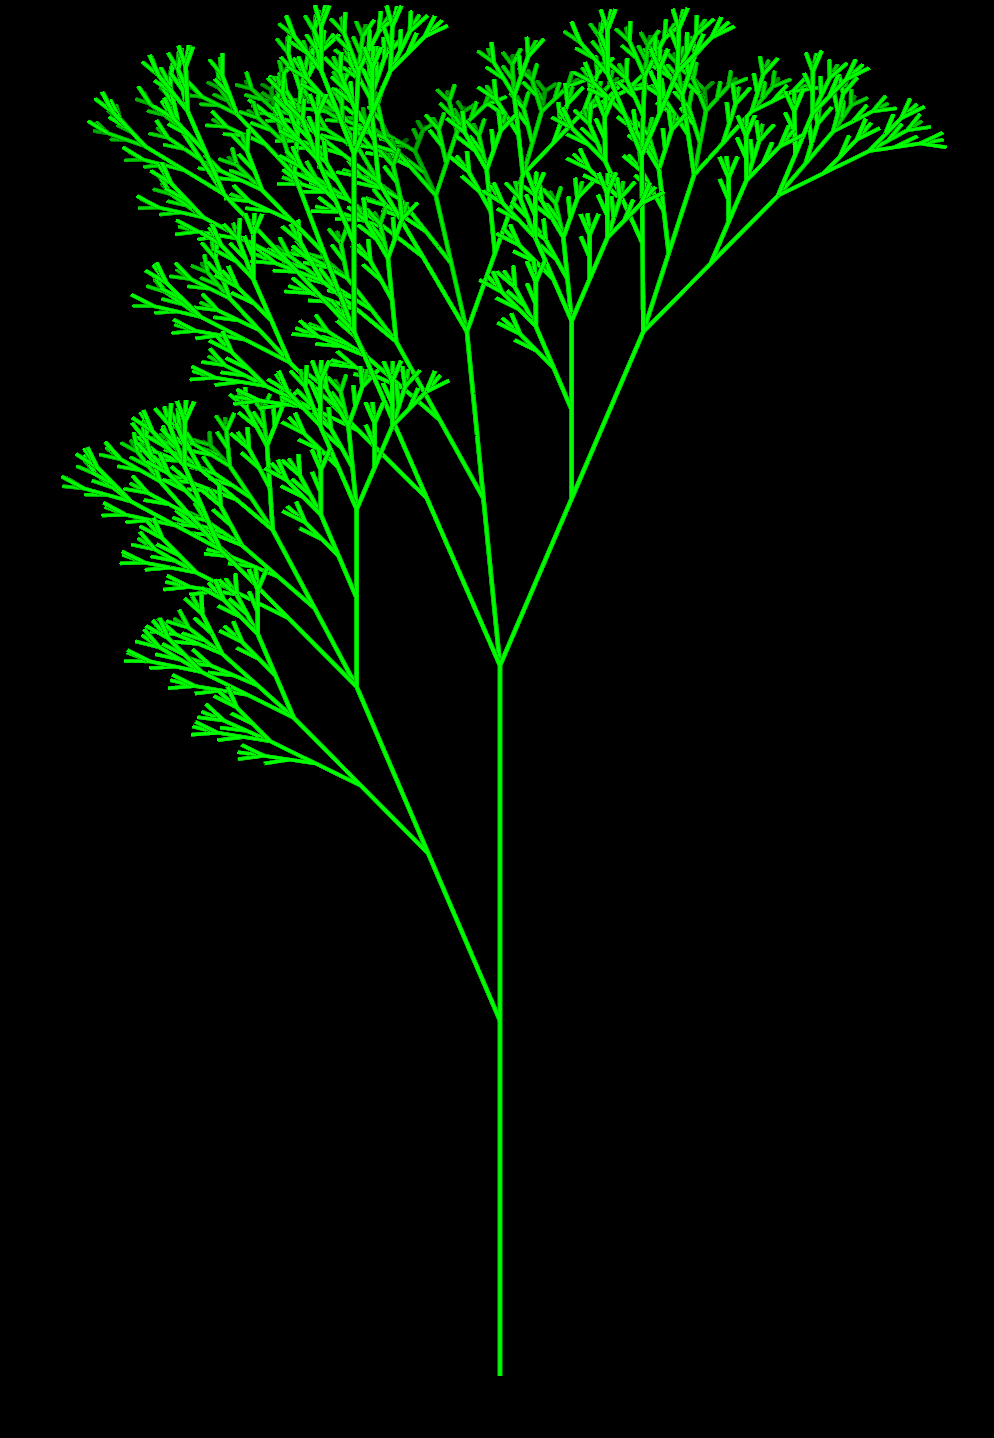
\includegraphics[scale=0.3]{images/tree-two.png}
        \caption{Arbre en 2D et Arbre en 3D}
        \label{fig:my_label}
    \end{figure}
    
	